\documentclass{lab_sheet}
\usepackage[flushleft]{threeparttable}
\usepackage[hidelinks]{hyperref}

\newcommand{\syntax}[1]{
    \lstinputlisting[label={lst:#1},caption={Syntax for configuring #1}, captionpos=b]{./Outputs/#1-syntax.txt}
}

\newcommand{\setting}[2]{
    \begin{tabular}{C{3cm}C{5cm}C{5cm}}
        \toprule
          #1 & IP address & Subnet mask\\
          \midrule
          #2
          \bottomrule
       \end{tabular}
}

\newcommand{\parameter}[1]{
    \begin{tabular}{C{3cm}C{2cm}C{2cm}C{2cm}C{2cm}}
        \toprule
        Router & hostname & console password & enable password& vty password\\
        \midrule
          #1 
          \bottomrule
       \end{tabular}
}

\newcommand{\customcaption}[2]{
    \begin{mdframed}[backgroundcolor=bg,innerbottommargin=-2.5em]
        \lstinputlisting[label={lst:#1},captionpos=b,style=DOS,caption={#2}]{./Outputs/#1.txt}
          \end{mdframed}
}
\newcommand{\ping}[1]{
    \begin{tabular}{||C{3cm}||C{5cm}||C{5cm}||}
        \toprule
          Sending Host & Destination & Ping status\\
          \hline
          #1
          \bottomrule
       \end{tabular}
}

\newcommand{\showroute}[1]{
  \foreach \i in {0,1,2,3}
  {
    \cmdop{#1-show\i}{show ip route on Router \i}
  }
}


\newcommand{\pingtest}[1]{
    \cmdop{#1-a}{ping test from PC0 to PC1}
    \cmdop{#1-b}{ping test from PC0 to PC2}
    \cmdop{#1-c}{ping test from PC1 to PC2}
    \cmdop{#1-d}{ping test from PC1 to PC3}
    \cmdop{#1-e}{ping test from PC2 to PC3}
    \cmdop{#1-f}{ping test from PC3 to PC0}
}

\newcommand{\tracert}[1]{
    \cmdop{#1-a0}{tracert from PC0 to PC1}
    \cmdop{#1-b0}{tracert from PC0 to PC2}
    \cmdop{#1-c0}{tracert from PC0 to PC3}

    \cmdop{#1-a1}{tracert from PC1 to PC0}
    \cmdop{#1-b1}{tracert from PC1 to PC2}
    \cmdop{#1-c1}{tracert from PC1 to PC3}

    \cmdop{#1-a2}{tracert from PC2 to PC0}
    \cmdop{#1-b2}{tracert from PC2 to PC1}
    \cmdop{#1-c2}{tracert from PC2 to PC3}

    \cmdop{#1-a3}{tracert from PC3 to PC0}
    \cmdop{#1-b3}{tracert from PC3 to PC1}
    \cmdop{#1-c3}{tracert from PC3 to PC2}
}

\begin{document}
\titlePage{Configuration of Dynamic Routing using RIP and OSPF}{December 10, 2020}
\pagenumbering{gobble}
\tableofcontents
\pagebreak
\listoffigures
\pagebreak
\listoftables
\pagebreak
\lstlistoflistings
\pagebreak
\pagenumbering{arabic}
\section{Objectives}
\begin{itemize}
	\item Familiarization with dynamic routing.
	\item Configuring dynamic routing using RIP and OSPF.
	\item Observe how dynamic routing can address changing network topology automatically.
\end{itemize}
\section{Required Tools}
\subsection{Cisco Packet Tracer}
Cisco Packet Tracer is a visual simulation software developed and distributed by Cisco Systems. Packet Tracer is a cross platform tool that allows simulated environment for modern computer network and network topologies.
\section{Simulation Activities}
\begin{figure}[H]
	\centering
	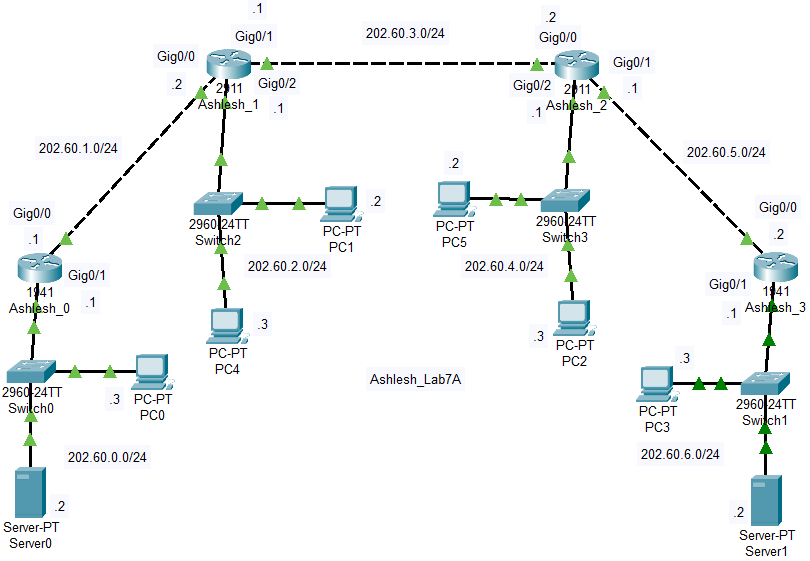
\includegraphics[scale=.8]{Figures/activitya.png}
	\caption{Simulated network for Activity A}
	\label{fig:activitya}
\end{figure}

\begin{figure}[H]
	\centering
	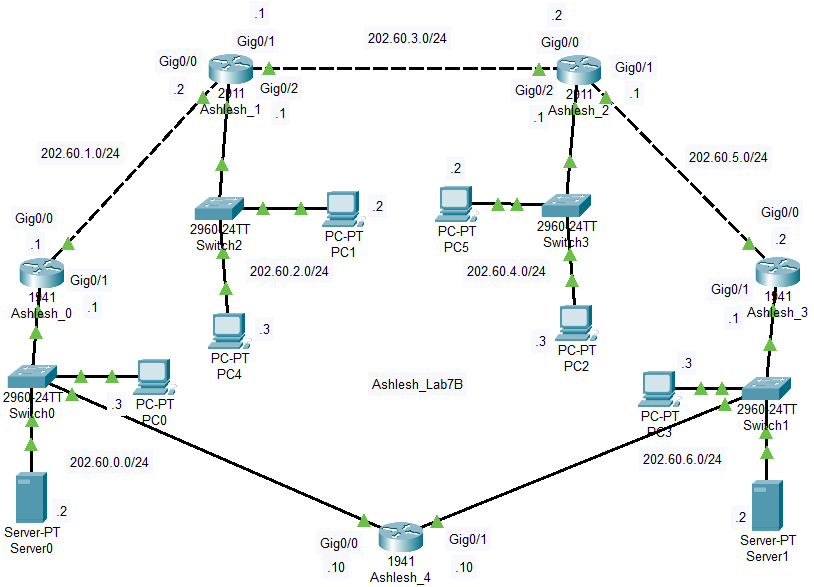
\includegraphics[scale=.8]{Figures/activityb.png}
	\caption{Simulated network for Activity B}
	\label{fig:activityb}
\end{figure}

\begin{figure}[H]
	\centering
	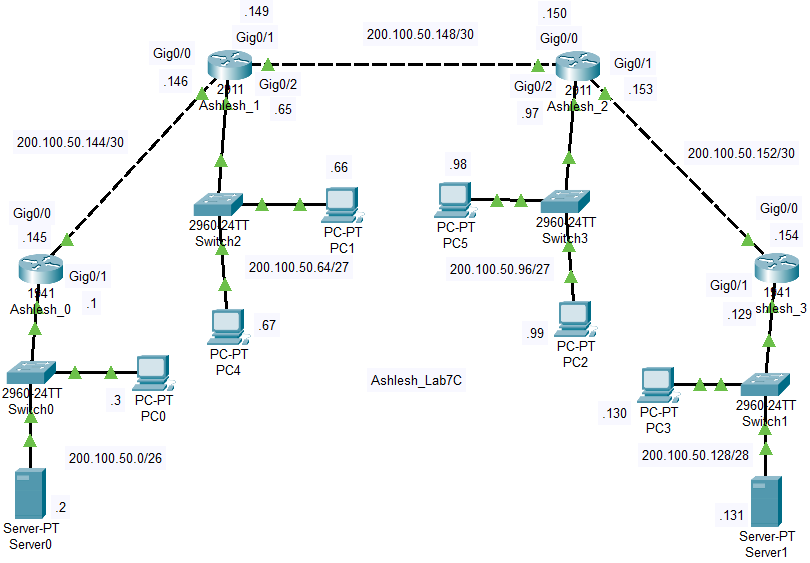
\includegraphics[scale=.8]{Figures/activityc.png}
	\caption{Simulated network for Activity C}
	\label{fig:activityc}
\end{figure}

\begin{figure}[H]
	\centering
	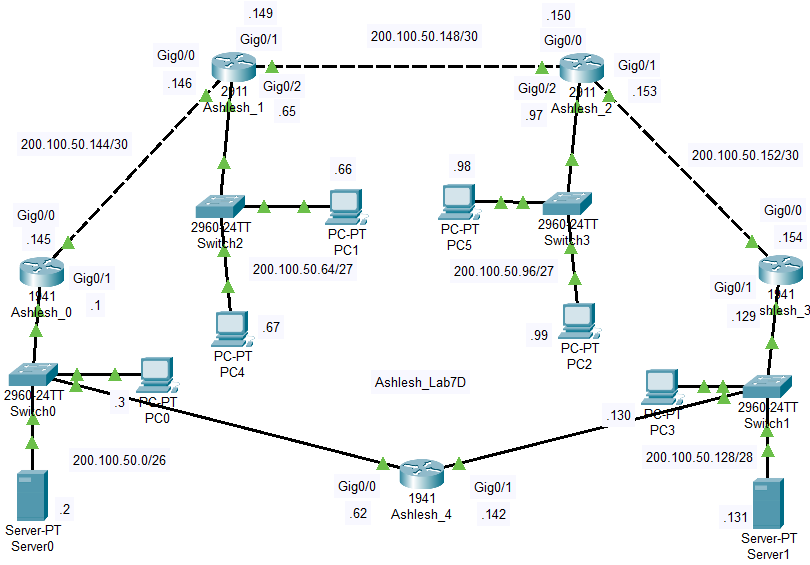
\includegraphics[scale=.8]{Figures/activityd.png}
	\caption{Simulated network for Activity D}
	\label{fig:activityd}
\end{figure}

\section{Exercises}
\problem{What is dynamic routing? How it differs with static routing? Explain briefly.}
Dynamic routing is a networking technique used for managing routing tables where updates in the network topologies are reflected in the routing table automatically. This is possible with the routing information being shared between adjacent routers such that any changes to the network are advertized according to the different protocols and are responsible for routing table updates.\\
It is different than static routing methods based on the following points,
\difference{Static Routing}{Dynamic Routing}{Difference}{
  Protocols used  & May not follow any protocol. & Follows protocols such as OSPF, RIP, BGP etc.\\
\hline
Adaptability & Routes are user defined, so don't adapt to network changes.& Routes adapt as per the changes in the network.\\
\hline
Security& Highly secure.& Less secure.\\
\hline
Applications& Smaller networks with less routes to be defined by the administrator. & Larger networks with frequently changing links.\\
\hline
Resources& No additional resources needed for application.   & Memory, bandwidth and other resources consumed during application.\\
\hline
Shortest path algorithm & Not applied.& Different algorithms based on protocols are applied for shortest route detection. \\
\hline
}
\problem{List out the dynamic routing configuration commands (used during the lab experiment) of router with their syntax and examples.}
\subsubsection*{RIP Configuration}
\syntax{RIP}
\subsubsection*{OSPF Configuration}
\syntax{OSPF}

\problem{Note down the observations of each steps with necessary commands specified in the activities mentioned in the lab sheet and comment on the result by explaining the reason in detail.}
To avoid repeated lines on the observations for \textit{show ip route} command, the codes for different kinds of routes are mentioned as,
\customcaption{codes}{Codes for different types of route included in show ip route}
\subproblem{Activity A}
\addtocontents{lol}{\protect\subsection*{Activity A}}
\addtocontents{lot}{\protect\subsection*{Activity A}}

\subsubsection*{Sub activity 1}
\addtocontents{lot}{\protect\subsubsection*{Sub activity 1}}

\begin{table}[H]
	\centering
	\parameter{
		0 & Ashlesh\_0 & \multirow{4}{*}{ashlesh} & \multirow{4}{*}{407} & \multirow{4}{*}{pandey}\\
		1 & Ashlesh\_1 & & & \\
		2 & Ashlesh\_2 & & & \\
		3 & Ashlesh\_3 & & & \\
	}
	\caption{Configuration parameters for routers}
	\label{tbl:parameter}
\end{table}


\subsubsection*{Sub activity 2}
\addtocontents{lot}{\protect\subsubsection*{Sub activity 2}}
\begin{table}[H]
	\centering
	\begin{threeparttable}
		\setting{Gigabitethernet interfaces}{
			Router 0: 0/0 & 202.60.1.1  & 255.255.255.0 \\
			Router 0: 0/1 & 202.60.0.1  & 255.255.255.0 \\
			Router 1: 0/0 & 202.60.1.2  & 255.255.255.0 \\
			Router 1: 0/1 & 202.60.3.1  & 255.255.255.0 \\
			Router 1: 0/2 & 202.60.2.1  & 255.255.255.0 \\
			Router 2: 0/0 & 202.60.3.2  & 255.255.255.0 \\
			Router 2: 0/1 & 202.60.5.1  & 255.255.255.0 \\
			Router 2: 0/2 & 202.60.4.1  & 255.255.255.0 \\
			Router 3: 0/0 & 202.60.5.2  & 255.255.255.0 \\
			Router 3: 0/1 & 202.60.6.1  & 255.255.255.0 \\
		}
		\begin{tablenotes}
			\small
			\item Note: The interfaces are marked on Figure~\ref{fig:activitya}.
		\end{tablenotes}
		\caption{IP address and subnet masks for the gigabitethernet interfaces on the routers}
		\label{tbl:gigasettingb}
	\end{threeparttable}
\end{table}

\subsubsection*{Sub activity 3}
\addtocontents{lot}{\protect\subsubsection*{Sub activity 3}}

\begin{table}[H]
	\centering
	\begin{threeparttable}
		\setting{Device}{
			PC0 & 202.60.0.3  & 255.255.255.0 \\
			PC1 & 202.60.2.2  & 255.255.255.0 \\
			PC2 & 202.60.4.3  & 255.255.255.0 \\
			PC3 & 202.60.6.3  & 255.255.255.0 \\
			PC4 & 202.60.2.3  & 255.255.255.0 \\
			PC5 & 202.60.4.2  & 255.255.255.0 \\
			Server0 & 202.60.0.2  & 255.255.255.0 \\
			Server1 & 202.60.6.2  & 255.255.255.0 \\
		}
		\begin{tablenotes}
			\small
			\item Note: The ip addressess and subnet masks are set using the IP configuration application. The default gateways for the PCs and servers were also set as, PC0 and Server0: 202.60.0.1, PC1 and PC4: 202.60.2.1, PC2 and PC5: 202.60.4.1, PC3 and Server1: 202.60.6.1
		\end{tablenotes}
		\caption{IP address and subnet masks for the PCs and servers in the network}
		\label{tbl:pcsettingb}
	\end{threeparttable}
\end{table}

\subsubsection*{Sub activity 4}
Telnet was enabled in sub activity 1 while configuring the vty terminal password.

\subsubsection*{Sub activity 5}
\addtocontents{lol}{\protect\subsubsection*{Sub activity 5}}
\showroute{a}

\subsubsection*{Sub activity 6}
\addtocontents{lot}{\protect\subsubsection*{Sub activity 6}}

\begin{table}[H]
    \centering
    \ping{
      \multirow{18}{*}{PC0} & PC0 & \multirow{2}{*}{Successful}\\
      & Server0 & \\
      \cline{2-3}
      & PC1 &  \multirow{6}{*}{Destination host unreachable}\\
      & PC4 &\\
      & PC2 &\\
      & PC5 &\\
      & PC3 &\\
      & Server1 & \\
      \cline{2-3}
      & Router0: 0/0 &  \multirow{2}{*}{Successful}\\
      & Router0: 0/1 & \\
      \cline{2-3}
      & Router1: 0/0 & Request timed out\\
      \cline{2-3}
      & Router1: 0/1 & \multirow{7}{*}{Destination host unreachable}\\
      & Router1: 0/2 & \\
      & Router2: 0/0 & \\
      & Router2: 0/1 & \\
      & Router2: 0/2 & \\
      & Router3: 0/0 & \\
      & Router3: 0/1 & \\
    }
\caption{Observation for ping tests from PC0 to other PCs, servers and router interfaces}
\label{tbl:activitya6}
\end{table}

\subsubsection*{Sub activity 7}
\addtocontents{lot}{\protect\subsubsection*{Sub activity 7}}
\begin{table}[H]
    \centering
    \ping{
      \multirow{18}{*}{PC1} & PC0 & \multirow{2}{*}{Destination host unreachable}\\
      & Server0 & \\
      \cline{2-3}
      & PC1 &  \multirow{2}{*}{Successful}\\
      & PC4 & \\
      \cline{2-3}
      & PC2 &\multirow{4}{*}{Destination host unreachable}\\
      & PC5 &\\
      & PC3 &\\
      & Server1 & \\
      \cline{2-3}
      & Router0: 0/0 & Request timed out\\
      \cline{2-3}
      & Router0: 0/1 & Destination host unreachable\\
      \cline{2-3}
      & Router1: 0/0 & \multirow{3}{*}{Successful}\\
      & Router1: 0/1 & \\
      & Router1: 0/2 & \\
      \cline{2-3}
      & Router2: 0/0 & Request timed out\\
      \cline{2-3}
      & Router2: 0/1 & \multirow{4}{*}{Destination host unreachable}\\
      & Router2: 0/2 & \\
      & Router3: 0/0 & \\
      & Router3: 0/1 & \\
    }
\caption{Observation for ping tests from PC1 to other PCs, servers and router interfaces}
\label{tbl:activitya7}
\end{table}

\subsubsection*{Sub activity 8}
\addtocontents{lot}{\protect\subsubsection*{Sub activity 8}}

\begin{table}[H]
    \centering
    \ping{
      \multirow{18}{*}{PC2} & PC0 & \multirow{4}{*}{Destination host unreachable}\\
      & Server0 & \\
      & PC1 & \\
      & PC4 & \\
      \cline{2-3}
      & PC2 &\multirow{2}{*}{Successful}\\
      & PC5 &\\
      \cline{2-3}
      & PC3 &\multirow{5}{*}{Destination host unreachable}\\
      & Server1 & \\
      & Router0: 0/0 & \\
      & Router0: 0/1 & \\
      & Router1: 0/0 & \\
      \cline{2-3}
      & Router1: 0/1 & Request timed out\\
      \cline{2-3}
      & Router1: 0/2 & Destination host unreachable\\
      \cline{2-3}
      & Router2: 0/0 & \multirow{3}{*}{Successful}\\
      & Router2: 0/1 & \\
      & Router2: 0/2 & \\
      \cline{2-3}
      & Router3: 0/0 & Request timed out\\
      \cline{2-3}
      & Router3: 0/1 & Destination host unreachable\\
    }
\caption{Observation for ping tests from PC2 to other PCs, servers and router interfaces}
\label{tbl:activitya8-2}
   \end{table}

   \begin{table}[H]
    \centering
    \ping{
      \multirow{18}{*}{PC3} & PC0 & \multirow{6}{*}{Destination host unreachable}\\
      & Server0 & \\
      & PC1 & \\
      & PC4 & \\
      & PC2 &\\
      & PC5 &\\
      \cline{2-3}
      & PC3 & \multirow{2}{*}{Successful}\\
      & Server1 & \\
      \cline{2-3}
      & Router0: 0/0 & \multirow{6}{*}{Destination host unreachable}\\
      & Router0: 0/1 & \\
      & Router1: 0/0 & \\
      & Router1: 0/1 & \\
      & Router1: 0/2 & \\
      & Router2: 0/0 & \\
      \cline{2-3}
      & Router2: 0/1 & Request timed out\\
      \cline{2-3}
      & Router2: 0/2 & Destination host unreachable\\
      \cline{2-3}
      & Router3: 0/0 & \multirow{2}{*}{Successful}\\
      & Router3: 0/1 & \\
    }
\caption{Observation for ping tests from PC3 to other PCs, servers and router interfaces}
\label{tbl:activitya8-3}
\end{table}

\begin{table}[H]
    \centering
    \ping{
      \multirow{16}{*}{Router 0} & PC0 & \multirow{2}{*}{Successful}\\
      & Server0 & \\
      \cline{2-3}
      & PC1 & \multirow{6}{*}{Failed}\\
      & PC4 & \\
      & PC2 &\\
      & PC5 &\\
      & PC3 &\\
      & Server1 & \\
      \cline{2-3}
      & Router1: 0/0 & Successful\\
      \cline{2-3}
      & Router1: 0/1 & \multirow{7}{*}{Failed}\\
      & Router1: 0/2 & \\
      & Router2: 0/0 & \\
      & Router2: 0/1 & \\
      & Router2: 0/2 & \\
      & Router3: 0/0 & \\
      & Router3: 0/1 & \\
    }
\caption{Observation for ping tests from Router 0 to other PCs, servers and router interfaces}
\label{tbl:activitya8-r0}
\end{table}

\begin{table}[H]
    \centering
    \ping{
      \multirow{15}{*}{Router 1} & PC0 & \multirow{2}{*}{Failed}\\
      & Server0 & \\
      \cline{2-3}
      & PC1 & \multirow{2}{*}{Successful}\\
      & PC4 & \\
      \cline{2-3}
      & PC2 &\multirow{4}{*}{Failed}\\
      & PC5 &\\
      & PC3 &\\
      & Server1 & \\
      \cline{2-3}
      & Router0: 0/0 & Successful\\
      \cline{2-3}
      & Router0: 0/1 & Failed \\
      \cline{2-3}
      & Router2: 0/0 & Successful\\
      \cline{2-3}
      & Router2: 0/1 & \multirow{4}{*}{Failed}\\
      & Router2: 0/2 & \\
      & Router3: 0/0 & \\
      & Router3: 0/1 & \\
    }
\caption{Observation for ping tests from Router 1 to other PCs, servers and router interfaces}
\label{tbl:activitya8-r1}
\end{table}

\begin{table}[H]
    \centering
    \ping{
      \multirow{15}{*}{Router 2} & PC0 & \multirow{4}{*}{Failed}\\
      & Server0 & \\
      & PC1 & \\
      & PC4 & \\
      \cline{2-3}
      & PC2 &\multirow{2}{*}{Successful}\\
      & PC5 &\\
      \cline{2-3}
      & PC3 &\multirow{2}{*}{Failed}\\
      & Server1 & \\
      \cline{2-3}
      & Router0: 0/0 & \multirow{3}{*}{Failed}\\
      & Router0: 0/1 &  \\
      & Router1: 0/0 & \\
      \cline{2-3}
      & Router1: 0/1 & Successful\\
      \cline{2-3}
      & Router1: 0/2 & Failed\\
      \cline{2-3}
      & Router3: 0/0 & Successful\\
      \cline{2-3}
      & Router3: 0/1 & Failed\\
    }
\caption{Observation for ping tests from Router 2 to other PCs, servers and router interfaces}
\label{tbl:activitya8-r2}
\end{table}


\begin{table}[H]
    \centering
    \ping{
      \multirow{16}{*}{Router 3} & PC0 & \multirow{6}{*}{Failed}\\
      & Server0 & \\
      & PC1 & \\
      & PC4 & \\
      & PC2 &\\
      & PC5 &\\
      \cline{2-3}
      & PC3 &\multirow{2}{*}{Successful}\\
      & Server1 & \\
      \cline{2-3}
      & Router0: 0/0 & \multirow{6}{*}{Failed}\\
      & Router0: 0/1 &  \\
      & Router1: 0/0 & \\
      & Router1: 0/1 & \\
      & Router1: 0/2 & \\
      & Router2: 0/0 & \\
      \cline{2-3}
      & Router2: 0/1 & Successful\\
      \cline{2-3}
      & Router2: 0/2 & Failed\\
    }
\caption{Observation for ping tests from Router 3 to other PCs, servers and router interfaces}
\label{tbl:activitya8-r3}
\end{table}

\subsubsection*{Sub activity 9}
\addtocontents{lol}{\protect\subsubsection*{Sub activity 9}}
\customcaption{a9-0}{Configuring RIP on Router 0 using telnet from PC0}

\subsubsection*{Sub activity 10}
\addtocontents{lol}{\protect\subsubsection*{Sub activity 10}}
\customcaption{a9-1}{Configuring RIP on Router 1 using telnet from Router 0}


\subsubsection*{Sub activity 11}
\addtocontents{lol}{\protect\subsubsection*{Sub activity 11}}
\customcaption{a9-2}{Configuring RIP on Router 2 using telnet from Router 1}
\customcaption{a9-3}{Configuring RIP on Router 3 using telnet from Router 2}

\subsubsection*{Sub activity 12}
\addtocontents{lol}{\protect\subsubsection*{Sub activity 12}}
\showroute{ar}
The routing tables shown in Listings~\ref{lst:ar-show0} to \ref{lst:ar-show3} are different than that in Listings~\ref{lst:a-show0} to \ref{lst:a-show3}. There are additional routes rather than just the local and connected ones. The routes configured using RIP are denoted with R in the table. Although only the adjacent networks were explicitly included during the RIP configuration, other networks are also learnt by individual routers with properly via links to these networks based on the neighbouring router's routing information. For instance, there are routes configured/learnt with RIP for all networks in Router 0 with the routes going through 202.60.1.2.

\pingtest{a6}
\begin{table}[H]
  \centering
  \ping{
    \multirow{18}{*}{\shortstack{PC0\\ \\or\\ \\PC1\\ \\or\\ \\PC2\\ \\or\\ \\PC3}} & PC0 & \multirow{18}{*}{Successful}\\
    & Server0 & \\
    & PC1 & \\
    & PC4 &\\
    & PC2 &\\
    & PC5 &\\
    & PC3 &\\
    & Server1 & \\
    & Router0: 0/0 & \\
    & Router0: 0/1 & \\
    & Router1: 0/0 & \\
    & Router1: 0/1 &\\
    & Router1: 0/2 & \\
    & Router2: 0/0 & \\
    & Router2: 0/1 & \\
    & Router2: 0/2 & \\
    & Router3: 0/0 & \\
    & Router3: 0/1 & \\
  }
\caption{Observation for ping tests from PC0, PC1, PC2 and PC3 to other PCs, servers and router interfaces}
\label{tbl:activityb17}
\end{table}

\begin{table}[H]
\centering
\ping{
  \multirow{16}{*}{Router 0} & PC0 & \multirow{16}{*}{Successful}\\
  & Server0 & \\
  & PC1 & \\
  & PC4 &\\
  & PC2 &\\
  & PC5 &\\
  & PC3 &\\
  & Server1 & \\
  & Router1: 0/0 & \\
  & Router1: 0/1 &\\
  & Router1: 0/2 & \\
  & Router2: 0/0 & \\
  & Router2: 0/1 & \\
  & Router2: 0/2 & \\
  & Router3: 0/0 & \\
  & Router3: 0/1 & \\
}
\caption{Observation for ping tests from Router 0 to other PCs, servers and router interfaces}
\label{tbl:activityb17r0}
\end{table}

\begin{table}[H]
\centering
\ping{
\multirow{15}{*}{Router 1} & PC0 & \multirow{15}{*}{Successful}\\
& Server0 & \\
& PC1 & \\
& PC4 &\\
& PC2 &\\
& PC5 &\\
& PC3 &\\
& Server1 & \\
& Router0: 0/0 & \\
& Router0: 0/1 & \\
& Router2: 0/0 & \\
& Router2: 0/1 & \\
& Router2: 0/2 & \\
& Router3: 0/0 & \\
& Router3: 0/1 & \\
}
\caption{Observation for ping tests from Router 1 to other PCs, servers and router interfaces}
\label{tbl:activityb17r1}
\end{table}

\begin{table}[H]
\centering
\ping{
\multirow{15}{*}{Router 2} & PC0 & \multirow{15}{*}{Successful}\\
& Server0 & \\
& PC1 & \\
& PC4 &\\
& PC2 &\\
& PC5 &\\
& PC3 &\\
& Server1 & \\
& Router0: 0/0 & \\
& Router0: 0/1 & \\
& Router1: 0/0 & \\
& Router1: 0/1 &\\
& Router1: 0/2 & \\
& Router3: 0/0 & \\
& Router3: 0/1 & \\
}
\caption{Observation for ping tests from Router 2 to other PCs, servers and router interfaces}
\label{tbl:activityb17r2}
\end{table}

\begin{table}[H]
\centering
\ping{
\multirow{16}{*}{Router 3} & PC0 & \multirow{16}{*}{Successful}\\
& Server0 & \\
& PC1 & \\
& PC4 &\\
& PC2 &\\
& PC5 &\\
& PC3 &\\
& Server1 & \\
& Router0: 0/0 & \\
& Router0: 0/1 & \\
& Router1: 0/0 & \\
& Router1: 0/1 &\\
& Router1: 0/2 & \\
& Router2: 0/0 & \\
& Router2: 0/1 & \\
& Router2: 0/2 & \\
}
\caption{Observation for ping tests from Router 3 to other PCs, servers and router interfaces}
\label{tbl:activityb17r3}
\end{table}

\subsubsection*{Sub activity 13}
\addtocontents{lol}{\protect\subsubsection*{Sub activity 13}}
\tracert{a13}

\subproblem{Activity B}
\addtocontents{lol}{\protect\subsection*{Activity B}}
A new router, Router 4 is added between Switch 0 and Switch 1 to increase reliability. The interfaces were configured as mentioned in Figure~\ref{fig:activityb}.
\customcaption{b-0}{Configuring RIP on Router 4 using CLI}

\subsubsection*{Sub activity 1}
\addtocontents{lol}{\protect\subsubsection*{Sub activity 1}}
\showroute{b}
The routing tables shown in Listings~\ref{lst:b-show0} to \ref{lst:b-show3} are different than that in Listings~\ref{lst:ar-show0} to \ref{lst:ar-show3}. There are additional routes for networks that go through the newly added router. For instance, there are two possible routes to the network 202.60.5.0/24 from Router 0, one through 202.60.1.2 and other through 202.60.0.10. This is due to the fact that both the routes have two hops in between the source and destination. In cases where one route has lesser hops than the other, only one of the routes is included. For instance, there is a route in Router 0's routing table to reach the network 202.60.6.0/24 that goes through 202.60.0.10. Although there is a possible lengthier route, it is removed once a route with lesser hops is detected.

\subsubsection*{Sub activity 2}
\addtocontents{lol}{\protect\subsubsection*{Sub activity 2}}
\tracert{b2}

\subsubsection*{Sub activity 3 [Removing link between Router 0 and Router 1]}
\addtocontents{lol}{\protect\subsubsection*{Sub activity 3 [Removing link between Router 0 and Router 1]}}
\tracert{b3}
\showroute{b3}

\subsubsection*{Sub activity 4 [Removing link between Router 1 and Router 2]}
\addtocontents{lol}{\protect\subsubsection*{Sub activity 4 [Removing link between Router 1 and Router 2]}}
\tracert{b4a}
\showroute{b4a}

\subsubsection*{Sub activity 4 [Removing link between Router 2 and Router 3]}
\addtocontents{lol}{\protect\subsubsection*{Sub activity 4 [Removing link between Router 2 and Router 3]}}
\tracert{b4b}
\showroute{b4b}

\subsubsection*{Sub activity 5}
From the observations mentioned in sub activity 4 of the activity B, with different links being removed we can see that the dynamic routing configuration automatically chooses the optimal path for the packets. In cases where link between two routers is down for some reason, the routing information from other routers enables the router under consideration to update it's own routing table such that the link that is down is avoided. This way, if any alternative route is available, it is included in the table and hence used by the packets. This way, addition of the router 4 such that there is an alternative route if the tested links are down, allows the packets to reach the destination. The observations for tracert also suggests that the packets take the route that isn't down based on the update in the routing tables of the routers.
\subproblem{Activity C}
\addtocontents{lol}{\protect\subsection*{Activity C}}
\addtocontents{lot}{\protect\subsection*{Activity C}}
\subsubsection*{Sub activity 1}
\addtocontents{lot}{\protect\subsubsection*{Sub activity 1}}

\begin{table}[H]
  \centering
  \begin{tabular}{|C{1cm}||C{1.5cm}||C{2.3cm}||C{2.3cm}||C{5cm}||C{1cm}|}
   \hline
   Subnet&Required Hosts&Network Address&Broadcast Address&
   Usable IP Addresses&Subnet Mask\\
   \hline
   A & 60 & 200.100.50.0 & 200.100.50.63 & 200.100.50.1~-~200.100.50.62 & /26\\
   \hline
   B & 27 & 200.100.50.64	 & 200.100.50.95 & 200.100.50.65~-~200.100.50.94 & /27\\
   \hline
   C & 25 & 200.100.50.96 & 200.100.50.127 & 200.100.50.97~-~200.100.50.126 & /27\\
   \hline
   D & 12 & 200.100.50.128 & 200.100.50.143 & 200.100.50.129~-~200.100.50.142 & /28\\
   \hline
   E & 2 & 200.100.50.144 & 200.100.50.147 & 200.100.50.145~-~200.100.50.146 & /30\\
   \hline
   F & 2 & 200.100.50.148 & 200.100.50.151 & 200.100.50.149~-~200.100.50.150 & /30\\
   \hline
   G & 2 & 200.100.50.152 & 200.100.50.155 & 200.100.50.153~-~200.100.50.154 & /30\\
   \hline
  \end{tabular}
  \caption{Subnet division as required by Activity C}
  \end{table}


\subsubsection*{Sub activity 2}
\addtocontents{lot}{\protect\subsubsection*{Sub activity 2}}

The gigabitethernet interfaces on the routers were set as,
\begin{table}[H]
	\centering
	\begin{threeparttable}
		\setting{Gigabitethernet interfaces}{
			Router 0: 0/0 & 200.100.50.145  & 255.255.255.252 \\
			Router 0: 0/1 & 200.100.50.1  & 255.255.255.192 \\
			Router 1: 0/0 & 200.100.50.146 & 255.255.255.252 \\
			Router 1: 0/1 & 200.100.50.149  & 255.255.255.252 \\
			Router 1: 0/2 & 200.100.50.65  & 255.255.255.224 \\
			Router 2: 0/0 & 200.100.50.150  & 255.255.255.252 \\
			Router 2: 0/1 & 200.100.50.153  & 255.255.255.252 \\
			Router 2: 0/2 & 200.100.50.97  & 255.255.255.224 \\
			Router 3: 0/0 & 200.100.50.154 & 255.255.255.252 \\
			Router 3: 0/1 & 200.100.50.129  & 255.255.255.240 \\
		}
		\begin{tablenotes}
			\small
			\item Note: The interfaces are marked on Figure~\ref{fig:activityc}.
		\end{tablenotes}
		\caption{IP address and subnet masks for the gigabitethernet interfaces on the routers}
		\label{tbl:gigasettingc}
	\end{threeparttable}
\end{table}

\begin{table}[H]
	\centering
	\begin{threeparttable}
		\setting{Device}{
			PC0 & 200.100.50.3  & 255.255.255.192 \\
			PC1 & 200.100.50.66 & 255.255.255.224 \\
			PC2 & 200.100.50.99  & 255.255.255.224 \\
			PC3 & 200.100.50.130 & 255.255.255.240 \\
			PC4 & 200.100.50.67  & 255.255.255.224 \\
			PC5 & 200.100.50.98  & 255.255.255.224 \\
			Server0 & 200.100.50.2  & 255.255.255.192 \\
			Server1 & 200.100.50.131  & 255.255.255.240 \\
		}
		\begin{tablenotes}
			\small
			\item Note: The ip addressess and subnet masks are set using the IP configuration application. The default gateways for the PCs and servers were also set as, PC0 and Server0: 200.100.50.1, PC1 and PC4: 200.100.50.65, PC2 and PC5: 200.100.50.97, PC3 and Server1: 200.100.50.129
		\end{tablenotes}
		\caption{IP address and subnet masks for the PCs and servers in the network}
		\label{tbl:pcsettingc}
	\end{threeparttable}
\end{table}

\subsubsection*{Sub activity 3}
\addtocontents{lot}{\protect\subsubsection*{Sub activity 3}}
\addtocontents{lol}{\protect\subsubsection*{Sub activity 3}}

\customcaption{c3-0}{Configuring OSPF on Router 0}
\customcaption{c3-1}{Configuring OSPF on Router 1}
\customcaption{c3-2}{Configuring OSPF on Router 2}
\customcaption{c3-3}{Configuring OSPF on Router 3}

\pingtest{c3}
\begin{table}[H]
  \centering
  \ping{
    \multirow{8}{*}{\shortstack{PC0\\ \\or\\ \\PC1\\ \\or\\ \\PC2\\ \\or\\ \\PC3}} & PC0 & \multirow{8}{*}{Successful}\\
    & Server0 & \\
    & PC1 & \\
    & PC4 &\\
    & PC2 &\\
    & PC5 &\\
    & PC3 &\\
    & Server1 & \\
  }
\caption{Observation for ping tests from PC0, PC1, PC2 and PC3 to other PCs and servers}
\label{tbl:activityc3}
\end{table}
\pagebreak
\subsubsection*{Sub activity 4}
\addtocontents{lol}{\protect\subsubsection*{Sub activity 4}}
\cmdop{c4}{tracert from PC0 to PC3}

\subsubsection*{Sub activity 5}
\addtocontents{lol}{\protect\subsubsection*{Sub activity 5}}
\showroute{c5}

\subproblem{Activity D}
\addtocontents{lol}{\protect\subsection*{Activity D}}
\subsubsection*{Sub activity 1}
\addtocontents{lol}{\protect\subsubsection*{Sub activity 1}}
A new router, Router 4 is added between Switch 0 and Switch 1 to increase reliability. The interfaces were configured as mentioned in Figure~\ref{fig:activityd}.
\customcaption{d1-0}{Configuring OSPF on Router 4}
\cmdop{d1-1}{tracert from PC3 to PC0}
\showroute{d1}

The routing tables shown in Listings~\ref{lst:d1-show0} to \ref{lst:d1-show3} are different than that in Listings~\ref{lst:c5-show0} to \ref{lst:c5-show3}. Additional OSPF routes are added to the routing tables. If there are multiple routes such that the number of intermediate hops is same, both are included in the table. If there are multiple routes, but one of them has the least hop, then only that is included in the table. Also, the additonal router 4 included in activity D reduces the hop from PC3 to PC0 such that the packet goes through the newly added router rather than the longer route through router 3. 

\subsubsection*{Sub activity 2 [Removing link between Router 4 and Switch 0]}
\addtocontents{lol}{\protect\subsubsection*{Sub activity 2 [Removing link between Router 4 and Switch 0]}}
\cmdop{d2-0}{tracert from PC3 to PC0}
\showroute{d2}
If the link between the router 4 and switch 0 is down for some reason, the packet takes the longer route through router 3 avoiding the damaged route. Since OSPF is a link state routing technique, the changes are reflected almost instantaneously. The routing tables are also updated accordingly. For instance, the router 0 now only has a route to the network 200.100.50.152 through 200.100.50.146 since the link 200.100.50.62 is down. This update is possible due to OSPF configurations on all the routers as mentioned.

\subsubsection*{Sub activity 3}
The observations are already included for none of the links being removed in Listings~\ref{lst:d1-1} to \ref{lst:d1-show3}.
\subsubsection*{Sub activity 4 [Removing link between Router 0 and Router 1]}
\addtocontents{lol}{\protect\subsubsection*{Sub activity 4 [Removing link between Router 0 and Router 1]}}
\tracert{d3a}
\showroute{d3a}

\subsubsection*{Sub activity 5 [Removing link between Router 1 and Router 2]}
\addtocontents{lol}{\protect\subsubsection*{Sub activity 5 [Removing link between Router 1 and Router 2]}}
\tracert{d3b}
\showroute{d3b}

\subsubsection*{Sub activity 5 [Removing link between Router 2 and Router 3]}
\addtocontents{lol}{\protect\subsubsection*{Sub activity 5 [Removing link between Router 2 and Router 3]}}
\tracert{d3c}
\showroute{d3c}
\problem{How dynamic routing can address the changing topology of a network automatically? Explain with reference to the observations.}
Dynamic routing, as the name suggests is used to dynamically change the routes based on changes in the network topology. Addition of new routes, or routes going out of service, both are handled automatically by dynamic routing. This is possible only if routers in the network can share their routing informations with other routers. This means that any changes detected by one router are reflected on other router's routing tables. \\[\baselineskip]
Based on the observations of this lab experiment, we can figure out how the two protocols RIP and OSPF operate. RIP works on distance vector algorithm, such that it uses a metric to determine the shortest path of any route. Any changes are broadcasted to all the neighbouring routers, and when a router receives a route that is not found in its own table, it updates the table to include the route. Further more, if there is a route present in its table that doesn't match its own, it keeps the shorter route in its table. This type of functioning is also known as rumor based routing. For OSPF, each router constructs its own map of the network based on updates from the neighbouring routers. Then, each router applies Dijkstra's algorithm to compute the shortest path to each destination network. This allows the changes to reflect almost instantly as observed. 
\section{Conclusion}
The activities provided in the lab sheet were performed in the given order that allowed us to understand the concepts of dynamic routing using RIP and OSPF protocols. While performing activity A, the concepts of RIP were dealt with in gist. The network topology was similar to the one we've already dealt, but this time the routing was handled dynamically rather than statically defining each route. This allowed us to realize the time and effort saved while using dynamic routing. A maximum of 3 RIP routes were included in the routers that represented the interfaces that were connected to different networks. The routing tables showed that other essential routes are automatically learnt by the routers based on the neighbouring router's routing information. Similarly, performing activity B allowed us to learn in depth about RIP routing, by disabling certain links in the network. Although some links were down in different observations, the connectivity wasn't lost, rather the router routed the packets through alternative routes automatically. This was a key observation since it wasn't possible in static routing. Moreover, performing the activity C allowed us to be familiar with OSPF routing protocol. Although the usage of different areas in the network wasn't dealt directly, the concepts were made clear. OSPF routing allowed the changes to be reflected almost instantaneously. During activity D, the addtion and removal of certain routes was visualized using Packet Tracer's simulation environment, which showed that packets were re-routed once a better route was added, or if the routes were out of service. The observations for this particular simulation couldn't be included in the report, however the inclusion of the packet tracer files cuts off the compromise made. Overall, the completion of this lab experiment allowes us to be familiar with concepts of dynamic routing using RIP and OSP, and also observe how dynamic routing handles changes in the network topology.
\end{document}